\documentclass[a4paper,12pt]{article}
\usepackage{polski}
\usepackage[utf8]{inputenc}
\usepackage[left = 3cm, right = 3cm, top = 2cm, bottom = 2cm]{geometry}
\usepackage{enumerate}
\usepackage{amssymb}		% pakiet do symboli
\usepackage{mathtools}		% pakiet do matmy (rozszerza amsmath)
\usepackage{enumitem}		% punktowanie (a), (b), ...
\usepackage{nopageno}		% brak numerow stron
\usepackage{graphicx}		% wstawianie obrazkow
\usepackage{float}			% wstawianie obrazkow w dowolnym miejscu
\usepackage{caption}
\usepackage{subcaption}
\usepackage{titling}
\usepackage{algpseudocode}	
\usepackage{algorithm}

% nowe komendy dla wygodniejszego pisania :)

\newcommand{\floor}[1]{\left\lfloor #1 \right\rfloor}	% podłoga
\newcommand{\ceil}[1]{\left\lceil #1 \right\rceil}		% sufit
\newcommand{\fractional}[1]{\left\{ #1 \right\}}		% część ułamkowa {x}
\newcommand{\set}[1]{\left \{ #1 \right \}}				% zbiór elementów {a,b,c}
\newcommand{\pair}[1]{\left( #1 \right)}				% para elementów (a,b)
\newcommand{\Mod}[1]{\ \mathrm{mod\ #1}}				% lekko zmodyfikowane modulo
\newcommand{\comp}[1]{\overline{ #1 }} 					% dopełnienie zbioru 
\DeclareMathOperator{\lcm}{lcm}							% obsługa lcm w mathmode

\begin{document}
\noindent \textbf{Matematyka dyskretna L, Lista 5 - Tomasz Woszczyński}\newline

\noindent \newline \textbf{Zadanie 1} \newline
Ile jest podzbiorów zbioru $n$ kolejnych liczb naturalnych, w których nie występują dwie kolejne liczby? \\ \\
Niech $A=\{x, x + 1, \dots, x + (n - 1) \}$, wtedy $|A| = n$. Rozpatrzmy podzbiory zbioru $A$ jako $n$-słowa (tzn. słowa binarne długości $n$) z alfabetu $\Sigma=\{0, 1\}$. \\
Przez $a_n$ oznaczmy liczbę dobrych podzbiorów, a więc takich, w których nie występują dwie kolejne liczby. Wtedy słowo może się rozpoczynać od "$0$" a pozostałe litery można do niego dodać na $a_{n-1}$ sposobów, lub zaczyna się od "$10$" i pozostałe litery dodajemy na $a_{n-2}$ sposobów. Stąd mamy, że
\[ a_n = a_{n-1} + a_{n-2} \]
a jego pierwszymi wyrazami są $a_1 = 2$ ("$0$", "$1$"), $a_2 = 3$ ("$00$", "$10$", "$01$"). \\
Można zauważyć więc, że ten ciąg będzie tworzył kolejne liczby Fibonacciego, a więc liczba szukanych podzbiorów to $a_n = F_{n+2}$.

\noindent \newline \textbf{Zadanie 2} \newline
Mamy policzyć ile jest liczb od $1$ do $800$, które są podzielne przez $6$ lub $8$, ale nie są podzielne przez $7$. \\ \\
Dla liczby $n \in \mathbb{N}_+$ jest $\floor{\frac{n}{a}}$ liczb podzielnych przez $a$.  Oznaczmy sobie zbiory liczb podzielnych przez $6$ jako $A$, przez $8$ jako $B$, a przez $7$ jako $C$. \\
Wiedząc, że $|A\cup B| = |A| + |B| - |A\cap B|$, interesować nas będzie wynik działania:
\[ \underbrace{|(A \cup B)|}_{\text{podzielne przez}\atop 6 \text{ lub } 8} - \underbrace{\underbrace{|(A \cap C)}_{\text{podzielne przez}\atop 6 \text{ i } 7} \cup \underbrace{(B \cap C)|}_{\text{podzielne przez}\atop 8 \text{ i } 7}}_{\text{podzielne przez } 6,\ 7,\ 8} \]
Rozpiszmy więc kolejne składniki działania:
\begin{align*}
&|(A \cup B)| = \floor{\frac{n}{6}} + \floor{\frac{n}{8}} - \floor{\frac{n}{\lcm(6, 8)}} = \floor{\frac{n}{6}} + \floor{\frac{n}{8}} - \floor{\frac{n}{24}} \stackrel{(n=800)}{=} 200\\
&|(A \cap C)| = \floor{\frac{n}{\lcm(6, 7)}} = \floor{\frac{n}{42}} \stackrel{(n=800)}{=} 19\\
&|(B \cap C)| = \floor{\frac{n}{\lcm(8, 7)}} = \floor{\frac{n}{56}} \stackrel{(n=800)}{=} 14\\
&|(A \cap C) \cup (B \cap C)| =  \floor{\frac{n}{\lcm(6, 7)}} + \floor{\frac{n}{\lcm(8, 7)}} - \floor{\frac{n}{\lcm(6, 7, 8)}} = \\
&=\floor{\frac{n}{42}} + \floor{\frac{n}{56}} - \floor{\frac{n}{168}} \stackrel{(n=800)}{=} 19 + 14 - 4 = 29
\end{align*}

\noindent Ostatecznym wynikiem jest więc $|(A \cup B)| - |(A \cap C) \cup (B \cap C)| = 200 - 29 = 171$.


\newpage
\noindent \textbf{Zadanie 4} \newline
Nieporządek to taka permutacja elementów, że żaden element nie znajduje się na swoim miejscu. Należy wyprowadzić wzór na liczbę nieporządków $d_n$ utworzonych z $n$ elementów korzystając z zasady włączeń i wyłączeń. \\ \\
Niech permutacja ma właściwość $P_i$ jeśli $i$-ty element znajduje się na $i$-tym miejscu. Szukać będziemy permutacji takich, dla których ta właściwość \textbf{nie jest} spełniona dla $i=1,2,\dots, n$. Niech $N = n!$ (liczba wszystkich permutacji). Mamy wtedy:
\begin{align*}
d_n &= N(\comp{P_1} \cup \comp{P_2} \cup \dots \cup \comp{P_n}) = \left| \bigcup\limits_{i=1}^{n} N(\comp{P_i}) \right| = \\
	&= N - \sum_{i}  N(P_i)  + \sum_{i < j}  N(P_i \cap P_j) - \sum_{i < j < k} N(P_i \cap P_j \cap P_k) + \\
	&\quad + \dots + (-1)^n\cdot N(P_1 \cap P_2 \cap \dots \cap P_n)
\end{align*}
Zauważmy, że $N(P_i) = (n - 1)!$, ponieważ $i$-ty element ma odgórnie wybraną pozycję a pozostałe $n - 1$ elementów są wybierane w dowolny sposób. Podobnie, dla $N(P_i \cap P_j)$ dwa elementy są na swoich miejscach, a wybierane są miejsca dla pozostałych $n-2$ elementów. W ogólności dla $m$ elementów mamy więc
\[ N(P_{i_1} \cap P_{i_2} \cap \dots \cap P_{i_m}) = (n - m)! \]
Ponadto możemy wybrać $m$ elementów z $n$-elementowego zbioru na $\binom{n}{m}$ sposobów. Rozpiszmy więc sumy z powyższego równania na $d_n$:
\begin{align*}
	\sum_{1 \leq i \leq n} N(P_i) &= \binom{n}{1} \cdot (n - 1)! \\
	\sum_{1 \leq i < j \leq n} N(P_i \cap P_j) &= \binom{n}{2} \cdot (n - 2)! \\
	&\hspace{0.5em} \vdots \\
	\sum_{1 \leq i_1 < \dots < i_m \leq n} N(P_{i_1} \cap P_{i_2} \cap \dots \cap P_{i_m}) &= \binom{n}{m} \cdot (n - m)! 
\end{align*}
Możemy więc podstawić obliczone sumy do wzoru na $d_n$, a następnie uprościć całość, aby otrzymać oczekiwany wzór na liczbę nieporządków $n$-elementowych:
\begin{align*}
	d_n &= n! - \binom{n}{1} \cdot (n - 1)! + \binom{n}{2} \cdot (n - 2)! - \dots + (-1)^n \cdot \binom{n}{n} \cdot (n - n)! = \\
		&= n! - \frac{n!}{1! (n - 1)!}\cdot (n - 1)! + \frac{n!}{2! (n - 2)!}\cdot (n - 2)! - \dots + (-1)^n \cdot \frac{n!}{n!0!}\cdot (n - n)! = \\
		&= n! \cdot \left[ 1 - \frac{1}{1!} + \frac{1}{2!} - \frac{1}{3!} + \dots + (-1)^n \cdot \frac{1}{n!} \right] \\
		&= n! \cdot \sum_{i=0}^{n} \frac{(-1)^i}{i!}
\end{align*}
Otrzymaliśmy więc wzór na liczbę nieporządków $n$-elementowych:
\[ d_n = n! \cdot \sum\limits_{i=0}^{n} \frac{(-1)^i}{i!} \]

\newpage
\noindent \textbf{Zadanie 7} \newline
Na płaszczyźnie jest $n$ okręgów, na ile maksymalnie obszarów mogą one podzielić tą płaszczyznę? Rozwiązanie należy wyprowadzić za pomocą zależności rekurencyjnej. \\ \\
Aby podzielić płaszczyznę na najwięcej obszarów przy użyciu $n$ okręgów muszą zostać spełnione dwa warunki:
\begin{enumerate}
	\item żaden z dwóch dowolnych okręgów nie leży wewnątrz innego,
	\item żadne trzy okręgi nie przecinają się w jednym miejscu.
\end{enumerate} 
Przez $r_n$ oznaczmy maksymalną liczbę obszarów, które możemy uzyskać za pomocą $n$ okręgów. Ilustrując pierwsze przypadki, możemy zobaczyć ile obszarów uzyskamy dla bardzo małych $n$:

\begin{figure}[H] % trzy rysunki przecinających się okręgów, wyśrodkowane w pionie
	\centering
	$\vcenter{\hbox{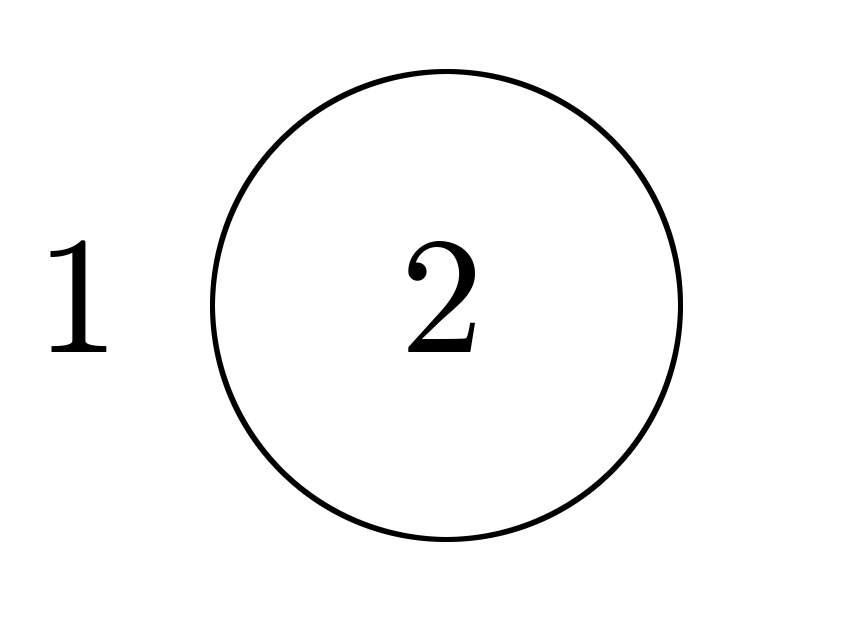
\includegraphics[width=.25\textwidth]{Rysunki/l5z7a.png}}}$
	$\vcenter{\hbox{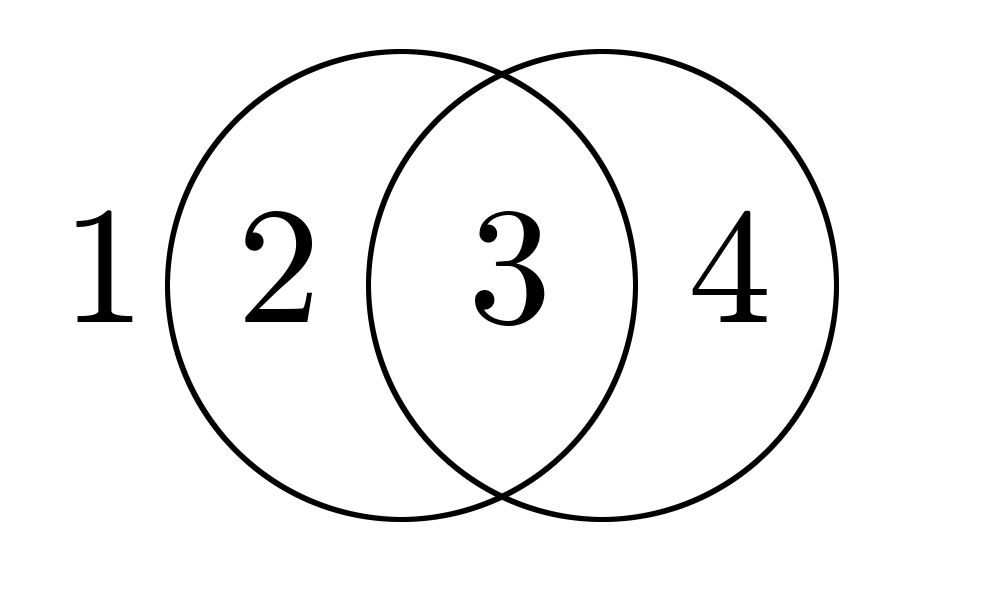
\includegraphics[width=.30\textwidth]{Rysunki/l5z7b.png}}}$
	$\vcenter{\hbox{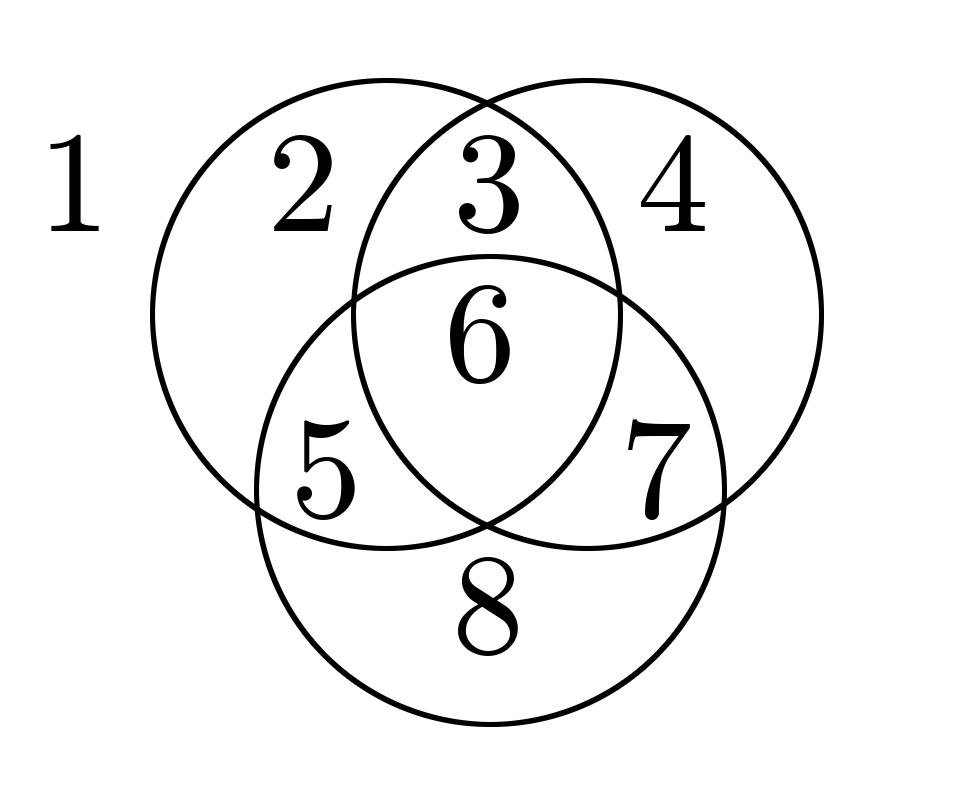
\includegraphics[width=.30\textwidth]{Rysunki/l5z7c.png}}}$
	\\ Rysunki przedstawiające podział płaszczyzny na obszary dla $n = 1, 2, 3$
\end{figure}
\noindent Na podstawie rysunków możemy stwierdzić, że $r_1 = 2, r_2 = 4, r_3 = 8$ -- dzięki temu będziemy mieli warunek początkowy oraz będziemy mogli sprawdzić czy otrzymana zależność rekurencyjna jest prawdziwa.\\ \\
Załóżmy, że mamy narysowane już $n - 1$ okręgów w najlepszym położeniu (tzn. tworzą najwięcej obszarów) i dodajemy do nich $n$-ty okrąg -- będzie się on przecinał z każdym z tych okręgów w $2$ miejscach. Każdy z $2(n - 1) = 2n - 2$ punktów dzieli $n$-ty okrąg na $2n - 2$ łuków. Każdy z tych łuków dzieli każdy z wcześniej istniejących regionów $r_{n-1}$ na dwa nowe. Otrzymujemy więc zależność rekurencyjną:
\[ 
r_n =
\begin{cases}
2 						&\text{ dla } n = 1 \\
r_{n - 1} + 2(n - 1) 	&\text{ dla } n \geq 2
\end{cases}
\]
Możemy to wyrażenie jeszcze uprościć, znajdując wzór jawny dla $r_n$:
\begin{align*}
	r_n &= r_{n - 1} + 2(n - 1) = \\
		&= r_{n - 2} + 2(n - 2) + 2(n - 1) = \\
		&= r_{n - 3} + 2(n - 3) + 2(n - 2) + 2(n - 1) = \\
		&= \ldots = \\
		&= r_1 + \sum\limits_{i = 1}^{n-1} 2(n - i) = r_1 + 2\cdot \sum\limits_{i = 1}^{n-1} (n - i) = \\
		&= 2 + 2 \cdot \underbrace{\left( \frac{(n - 1)\cdot n}{2} \right)}_{1 + 2 + \ldots + (n - 1)} = n^2 - n + 2 \text{ dla } n \geq 0
\end{align*}

\newpage
\noindent \textbf{Zadanie 8} \newline
Na ile maksymalnie obszarów można podzielić trójwymiarową przestrzeń $\mathbb{R}^3$ za pomocą $n$ płaszczyzn? Należy wyprowadzić zależność rekurencyjną.\\

\noindent Rozpatrzmy najpierw na ile obszarów można podzielić płaszczyznę $\mathbb{R}^2$ używając do tego $n$ linii. Niech $p_n$ oznacza maksymalną liczbę obszarów uzyskanych $n$ cięciami, wtedy $p_0 = 1$ (brak cięć), $p_1 = 2$ (jedno cięcie), $p_2 = 4$, itd. \\

\noindent Załóżmy, że mamy narysowane $n - 1$ linii (nierównoległych, przecinających się w największej ilości punktów). Rysując $n$-tą linię powstanie $n - 1$ nowych punktów przecięcia, które dzielą linię $n$-tą na $n$ części. Oznacza to, że do $p_{n-1}$ regionów dodane zostanie $n$ nowych regionów. Opisuje to zależność rekurencyjna:
\[ 
p_n =
\begin{cases}
1 			&\text{ dla } n = 0 \\
p_{n-1} + n &\text{ dla } n \geq 1
\end{cases}
\]
Wzór jawny zależności rekurencyjnej $p_n$:
\begin{align*}
	p_n &= p_{n-1} + n = \\
		&= p_{n-2} + n + (n - 1) = \\
		&= p_{n-3} + n + (n - 1) + (n - 2) = \\
		&= \ldots = \\
		&= p_0 + n + (n - 1) + \ldots + 1 = \\
		&= 1 + \sum\limits_{i = 1}^{n} i = 1 + \frac{n\cdot (n + 1)}{2} \text{ dla } n \geq 0
\end{align*}

\noindent Teraz możemy przejść do $\mathbb{R}^3$ i uogólnić rozważania nad przecinaniem płaszczyzny do przecinania przestrzeni. W tym przypadku warto zauważyć, że dwie przecinające się płaszczyzny mogą się przeciąć jedynie na jednej linii.
\begin{figure}[H]
	\centering
	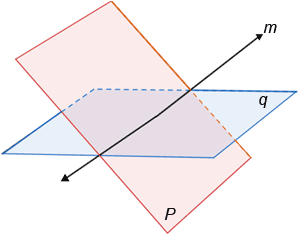
\includegraphics[width=0.35\textwidth]{Rysunki/l5z8.png}
	\\ Płaszczyzny $p$ oraz $q$ przecinają się tylko w jednej linii $m$
\end{figure}

\noindent Niech $q_n$ oznacza maksymalną liczbę obszarów stworzonych przez $n$ przecinających się płaszczyzn. Jasne jest, że $q_0 = 1$, jako że nie wykonujemy żadnego cięcia i przestrzeń jest nienaruszona, a kolejne wyrazy to $q_1 = 2$, $q_2 = 4$, $q_3 = 8$, itd. \\ 

\noindent Podobnie jak w przypadku cięć liniami, $n$-ta płaszczyzna przetnie $n - 1$ płaszczyzn w maksymalnie $n - 1$ liniach, a więc utworzy $n - 1$ nowych linii (tworzących $p_{n-1}$ obszarów). Oznacza to, że do $q_{n-1}$ obszarów zostanie dodanych $p_{n-1}$ obszarów stworzonych przez linie. Wyraża to zależność rekurencyjna:
\[ 
q_n = 
\begin{cases}
1 																	&\text{ dla } n = 0 \\
q_{n - 1} + p_{n - 1} = q_{n - 1} + 1 + \frac{n\cdot (n - 1)}{2} 	&\text{ dla } n \geq 1
\end{cases}
\]

\noindent Można jeszcze wyprowadzić wzór jawny:
\begin{align*}
	q_n &= q_{n - 1} + p_{n - 1} = q_{n - 1} + \underbrace{1 + \frac{n\cdot (n - 1)}{2}}_{p_{n-1}} = \\
		&= q_{n - 2} + \underbrace{1 + \frac{n\cdot (n - 1)}{2}}_{p_{n-1}} + \underbrace{1 + \frac{(n - 1)\cdot (n - 2)}{2}}_{p_{n-2}} = \\
		&= \ldots = \\
		&= q_0 + \sum\limits_{i = 0}^{n - 1} 1 + \underbrace{\sum\limits_{i = 0}^{n - 1} \underbrace{\frac{i \cdot (i + 1)}{2}}_{\mathclap{i\text{-ta liczba trójkątna}}}}_{\mathclap{n-1 \text{-ta liczba czworościenna}}} \\
		&= 1 + n + \frac{(n - 1)\cdot n \cdot(n + 1)}{6} = \\
		&= 1 + n + \frac{n^3 - n}{6} = \frac{n^3 + 5n + 6}{6} \text{ dla } n \geq 0
\end{align*}
\noindent Wyjaśnienie: $i$-ta \textit{liczba trójkątna} to suma liczb od $1$ do $i$ $\left(\frac{n \cdot (n + 1)}{2}\right)$, a $j$-ta \textit{liczba czworościenna} to suma liczb trójkątnych od $1$ do $j$, wyraża się ją wzorem $\frac{n\cdot(n+1)\cdot(n+2)}{6}$.


\noindent \newline \textbf{Zadanie 10} \newline
Na ile sposobów można wejść po schodach zbudowanych z $n$ stopni, jeśli w każdym kroku można pokonać jeden lub dwa stopnie? \\

\noindent Na pierwszy schodek można wejść tylko na $1$ sposób, na drugi na $2$ (dwa małe kroki lub jeden duży). Wejść na $n$-ty stopień można albo ze schodka $n-1$ albo z $n-2$ (dystans odpowiednio jednego lub dwóch schodków). Oznacza to, że liczba możliwości wejścia na $n$-ty schodek wyraża się zależnością rekurencyjną:
\[ 
x_n =
\begin{cases}
1 					&\text{ dla } n = 1\\
2 					&\text{ dla } n = 2\\
x_{n-1} + x_{n-2}	&\text{ dla } n \geq 3\\
\end{cases}
\]
\noindent Można zauważyć, że są to kolejne liczby Fibonacciego, a dokładniej $x_n = F_{n+1}$, więc na $n$-ty schodek można wejść na $F_{n+1}$ sposobów.

\end{document}